\documentclass{article}

\usepackage{graphicx}
\usepackage{tikz}
\usepackage{tikzsymbols}
\usetikzlibrary{calc,patterns,shapes.geometric}
\pagestyle{empty}
\usepackage[margin=0pt]{geometry}
\geometry{papersize={14in,12in}}

\def\centerarc[#1](#2)(#3:#4:#5){\draw[#1] ($(#2)+({#5*cos(#3)},{#5*sin(#3)})$) arc (#3:#4:#5);}

\begin{document}
	\begin{figure}
		\centering
		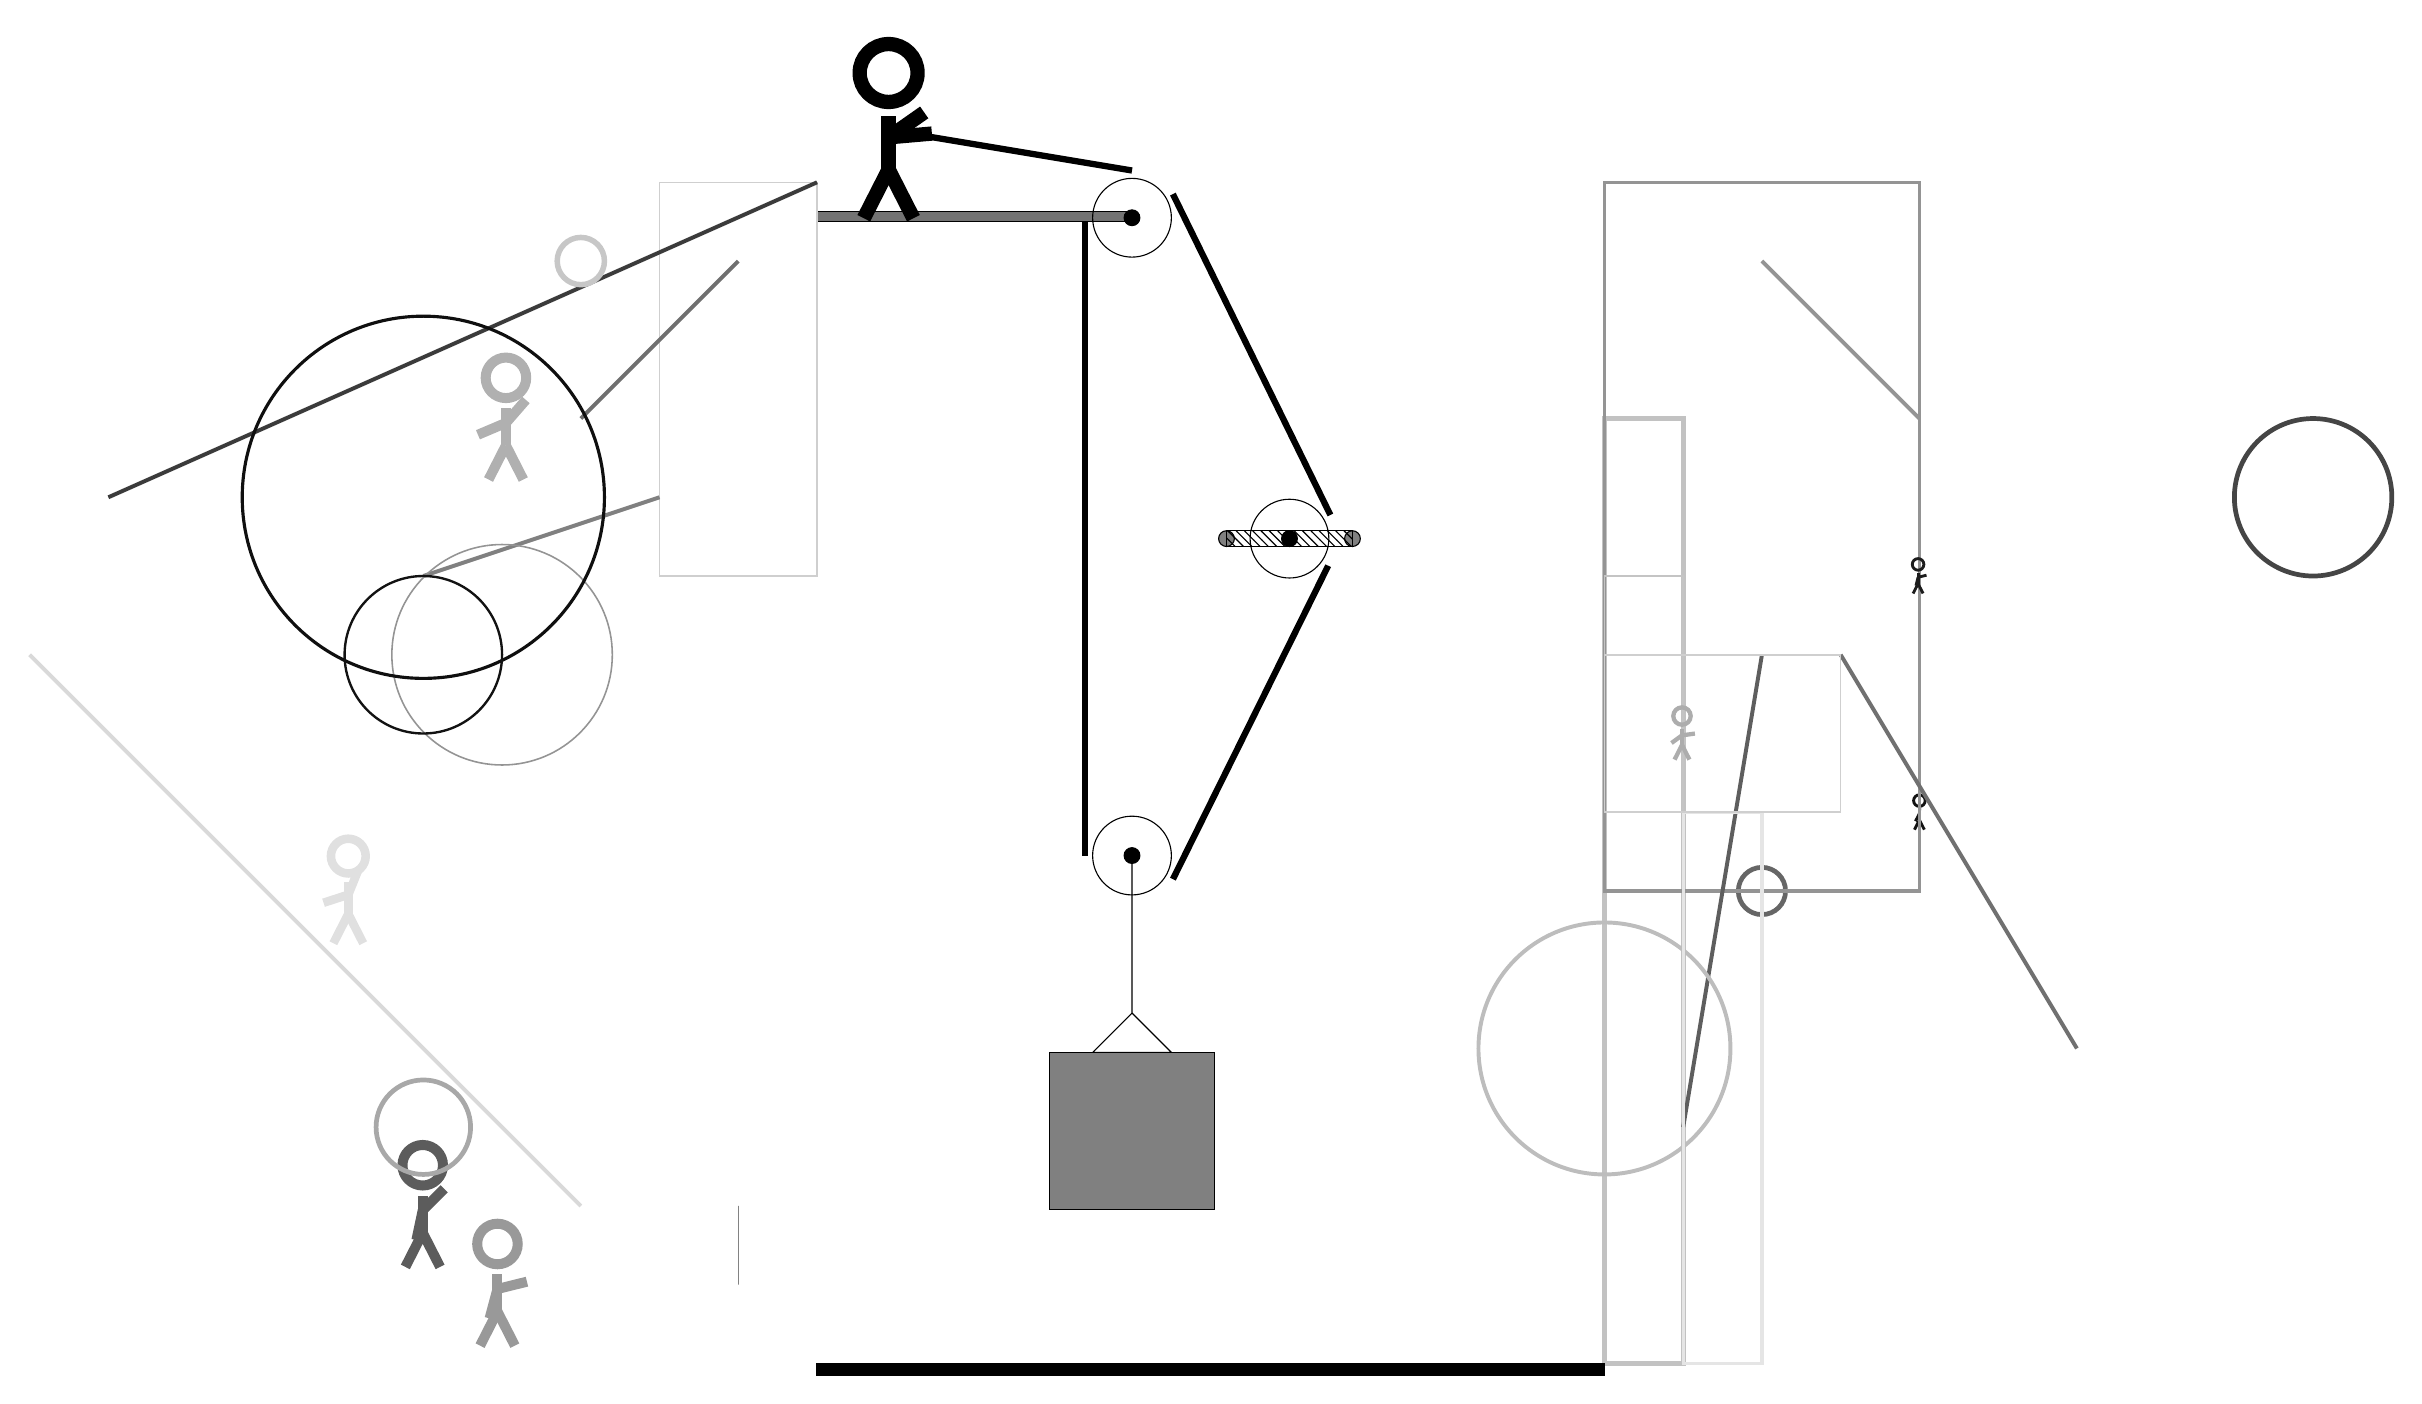
\begin{tikzpicture}
			%%%%% START %%%%%
			
			\draw[fill=black!55] (-2, 11.5) rectangle (2, 11.625);
			
			\draw (2, 3.45) circle (0.5);
			\draw[fill=black] (2, 3.45) circle (0.1);
			
			\draw (2, 11.55) circle (0.5);
			\draw[fill=black] (2, 11.55) circle (0.1);
			
			\draw[fill=white](4, 7.475) circle (0.5);
			\draw[fill=black] (4, 7.475) circle (0.1);
			\draw[fill=black!50] (3.2, 7.475) circle (0.1);
			\draw[fill=black!50] (4.8, 7.475) circle (0.1);
			\draw[pattern=north west lines, pattern color=black] (3.2, 7.575) rectangle (4.8, 7.375);
			
			\draw (2, 3.45) -- (2, 1.45) -- (1.5, 0.95) -- (2.5, 0.95) -- (2, 1.45);
			\draw[fill=black!50] (0.95, 0.95) rectangle (3.05, -1.05);
			
			\draw[line width=0.8mm] (1.4, 11.5) -- (1.4, 3.45);
			\centerarc[line width=0.8mm](2, 3.45)(180:330:0.6);
			\draw[line width=0.8mm](2.5196, 3.15) -- (4.4915, 7.1308);
			\centerarc[line width=0.8mm](4, 7.475)(390:325:0.6);
			\draw[line width=0.8mm](4.5196, 7.775) -- (2.5196, 11.85);
			\centerarc[line width=0.8mm](2, 11.55)(30:90:0.6);
			\draw[line width=0.8mm](2, 12.15) -- (-1, 12.65);
			
			\node at (-1, 12.65) {\Strichmaxerl[10][-175][35]};
			
			\draw[line width=0.2mm, color=black!19] (-2, 12) rectangle (-4, 7);
			
			\draw[line width=0.5mm, color=black!56](-5, 9) -- (-3, 11);
			\draw[line width=0.5mm, color=black!42](10, 11) -- (12, 9);
			\draw[line width=0.5mm, color=black!50](-4, 8) -- (-7, 7);
			\node[line width=0.7mm, color=black!64] at (-7, -1) {\Strichmaxerl[7][78][45]};
			\draw[line width=0.6mm, color=black!24] (9, 9) rectangle (8, -3);
			\node[line width=0.4mm, color=black!93] at (12, 4) {\Strichmaxerl[2][63][87]};
			\draw [line width=0.6mm, color=black!60](10, 3) circle (0.3);
			\node[line width=0.6mm, color=black!31] at (-6, 9) {\Strichmaxerl[7][23][49]};
			\draw[line width=0.5mm, color=black!15](-5, -1) -- (-12, 6);
			\draw[line width=0.4mm, color=black!42] (8, 12) rectangle (12, 3);
			\draw[line width=0.5mm, color=black!63](9, 0) -- (10, 6);
			\draw [line width=0.2mm, color=black!42](-6, 6) circle (1.4);
			
			\draw [line width=0.5mm, color=black!26](8, 1) circle (1.6);
			\draw[line width=0.5mm, color=black!56](11, 6) -- (14, 1);
			\draw[line width=0.5mm, color=black!77](-2, 12) -- (-11, 8);
			
			\draw [line width=0.6mm, color=black!73](17, 8) circle (1.0);
			\draw [line width=0.4mm, color=black!94](-7, 8) circle (2.3);
			\draw [line width=0.7mm, color=black!22](-5, 11) circle (0.3);
			\node[line width=0.4mm, color=black!89] at (12, 7) {\Strichmaxerl[2][76][14]};
			\draw [line width=0.3mm, color=black!93](-7, 6) circle (1.0);
			\draw[line width=0.2mm, color=black!49] (-3, -1) rectangle (-3, -2);
			\draw[line width=0.2mm, color=black!23] (9, 4) rectangle (8, 7);
			\draw [line width=0.6mm, color=black!34](-7, 0) circle (0.6);
			\node[line width=0.7mm, color=black!12] at (-8, 3) {\Strichmaxerl[6][18][68]};
			
			\node[line width=0.2mm, color=black!40] at (-6, -2) {\Strichmaxerl[7][75][14]};
			\node[line width=0.2mm, color=black!32] at (9, 5) {\Strichmaxerl[3][36][8]};
			\draw[line width=0.4mm, color=black!10] (10, 4) rectangle (9, -3);
			\draw[line width=0.2mm, color=black!19] (8, 4) rectangle (11, 6);
			
			\draw[fill=black] (-2, -3) rectangle (8, -3.15);
			
			%%%%% END %%%%%
		\end{tikzpicture}
	\end{figure}	
\end{document}